\documentclass[11pt,]{article}
\usepackage{lmodern}
\usepackage{amssymb,amsmath}
\usepackage{ifxetex,ifluatex}
\usepackage{fixltx2e} % provides \textsubscript
\ifnum 0\ifxetex 1\fi\ifluatex 1\fi=0 % if pdftex
  \usepackage[T1]{fontenc}
  \usepackage[utf8]{inputenc}
\else % if luatex or xelatex
  \ifxetex
    \usepackage{mathspec}
  \else
    \usepackage{fontspec}
  \fi
  \defaultfontfeatures{Ligatures=TeX,Scale=MatchLowercase}
\fi
% use upquote if available, for straight quotes in verbatim environments
\IfFileExists{upquote.sty}{\usepackage{upquote}}{}
% use microtype if available
\IfFileExists{microtype.sty}{%
\usepackage{microtype}
\UseMicrotypeSet[protrusion]{basicmath} % disable protrusion for tt fonts
}{}
\usepackage[margin=1.0in]{geometry}
\usepackage{hyperref}
\hypersetup{unicode=true,
            pdftitle={Specific taxa differentiate proximal and distal microbiota in the unprepped human colon},
            pdfborder={0 0 0},
            breaklinks=true}
\urlstyle{same}  % don't use monospace font for urls
\usepackage{graphicx,grffile}
\makeatletter
\def\maxwidth{\ifdim\Gin@nat@width>\linewidth\linewidth\else\Gin@nat@width\fi}
\def\maxheight{\ifdim\Gin@nat@height>\textheight\textheight\else\Gin@nat@height\fi}
\makeatother
% Scale images if necessary, so that they will not overflow the page
% margins by default, and it is still possible to overwrite the defaults
% using explicit options in \includegraphics[width, height, ...]{}
\setkeys{Gin}{width=\maxwidth,height=\maxheight,keepaspectratio}
\IfFileExists{parskip.sty}{%
\usepackage{parskip}
}{% else
\setlength{\parindent}{0pt}
\setlength{\parskip}{6pt plus 2pt minus 1pt}
}
\setlength{\emergencystretch}{3em}  % prevent overfull lines
\providecommand{\tightlist}{%
  \setlength{\itemsep}{0pt}\setlength{\parskip}{0pt}}
\setcounter{secnumdepth}{0}
% Redefines (sub)paragraphs to behave more like sections
\ifx\paragraph\undefined\else
\let\oldparagraph\paragraph
\renewcommand{\paragraph}[1]{\oldparagraph{#1}\mbox{}}
\fi
\ifx\subparagraph\undefined\else
\let\oldsubparagraph\subparagraph
\renewcommand{\subparagraph}[1]{\oldsubparagraph{#1}\mbox{}}
\fi

%%% Use protect on footnotes to avoid problems with footnotes in titles
\let\rmarkdownfootnote\footnote%
\def\footnote{\protect\rmarkdownfootnote}

%%% Change title format to be more compact
\usepackage{titling}

% Create subtitle command for use in maketitle
\newcommand{\subtitle}[1]{
  \posttitle{
    \begin{center}\large#1\end{center}
    }
}

\setlength{\droptitle}{-2em}
  \title{\emph{Specific taxa differentiate proximal and distal microbiota in the
unprepped human colon}}
  \pretitle{\vspace{\droptitle}\centering\huge}
  \posttitle{\par}
  \author{}
  \preauthor{}\postauthor{}
  \date{}
  \predate{}\postdate{}


\begin{document}
\maketitle

\vspace{35mm}

Running title: Specific taxa differentiate proximal and distal human
colon microbiota

\vspace{35mm}

Kaitlin J. Flynn\textsuperscript{1}, Charles C.
Koumpouras\textsuperscript{1}, Mack T. Ruffin IV\textsuperscript{2},
Danielle Kimberly Turgeon\textsuperscript{3}, and Patrick D.
Schloss\textsuperscript{1\(\dagger\)}

\vspace{35mm}

\(\dagger\) Corresponding author:
\href{mailto:pschloss@umich.edu}{\nolinkurl{pschloss@umich.edu}}

1. Department of Microbiology and Immunology, University of Michigan
Medical School, Ann Arbor, Michigan 48109

2. Pennslyvania State University, Hershey, Pennslyvania ??

3. Department of Internal Medicine, Division of Gastroenterology,
University of Michigan Medical School, Ann Arbor, Michigan

\newpage

\linenumbers

\begin{verbatim}
## randomForest 4.6-12
\end{verbatim}

\begin{verbatim}
## Type rfNews() to see new features/changes/bug fixes.
\end{verbatim}

\begin{verbatim}
## 
## Attaching package: 'ggplot2'
\end{verbatim}

\begin{verbatim}
## The following object is masked from 'package:randomForest':
## 
##     margin
\end{verbatim}

\begin{verbatim}
## Type 'citation("pROC")' for a citation.
\end{verbatim}

\begin{verbatim}
## 
## Attaching package: 'pROC'
\end{verbatim}

\begin{verbatim}
## The following objects are masked from 'package:stats':
## 
##     cov, smooth, var
\end{verbatim}

\begin{verbatim}
## 
## Attaching package: 'dplyr'
\end{verbatim}

\begin{verbatim}
## The following object is masked from 'package:randomForest':
## 
##     combine
\end{verbatim}

\begin{verbatim}
## The following objects are masked from 'package:stats':
## 
##     filter, lag
\end{verbatim}

\begin{verbatim}
## The following objects are masked from 'package:base':
## 
##     intersect, setdiff, setequal, union
\end{verbatim}

\begin{verbatim}
## AUCRF 1.1
\end{verbatim}

\begin{verbatim}
## Loading required package: lattice
\end{verbatim}

\begin{verbatim}
## 
## Attaching package: 'reshape2'
\end{verbatim}

\begin{verbatim}
## The following object is masked from 'package:tidyr':
## 
##     smiths
\end{verbatim}

\subsubsection{Abstract}\label{abstract}

Colorectal cancer (CRC) remains a leading cause of death worldwide
despite improved preventative and therapeutic measures. Tumors of the
proximal (right) and distal (left) colon are morphologically and
genetically distinct. Previous work from our group found that microbial
dysbiosis is associated with the development of CRC tumors in studies of
both mice and humans. Analysis of the fecal microbiota from healthy and
CRC patients further revealed different microbial signatures associated
with disease. We extended our observations of the fecal microbiome to
include analysis of the proximal and distal human colon. We used a
two-colonoscope approach on subjects that had not undergone standard
bowel preparation procedure. This technique allowed us to characterize
the native proximal and distal luminal and mucosal microbiome without
prior chemical disruption. 16S rRNA gene sequencing was performed on
proximal and distal mucosal and luminal biopsies and home-collected
stool for 20 healthy individuals. Diversity analysis revealed that each
site contained a diverse community, and that a patient's samples were
more similar to each other than to that of other individuals. Since we
could not differentiate sites along the colon based on community
structure or community membership alone, we employed the Random Forest
machine-learning algorithm to identify key species that distinguish
biogeographical sites. Random Forest classification models were built
using taxa abundance and sample location and revealed distinct
populations that were found in each location. \emph{Peptoniphilus,
Anaerococcus, Enterobacteraceae, Pseudomonas} and \emph{Actinomyces}
were most likely to be found in mucosal samples versus luminal samples
(AUC = 0.925). The classification model performed well (AUC = 0.912)
when classifying mucosal samples into proximal or distal sides, but
separating luminal samples from each side proved more challenging (AUC =
0.755). The left mucosa was found to have high populations of
\emph{Finegoldia, Murdochiella} and \emph{Porphyromonas}. Proximal and
distal luminal samples were comprised of many of the same taxa, likely
reflecting the fact that stool moves along the colon from the proximal
to distal end. Finally, comparison of all samples to fecal samples taken
at exit uncovered that the feces were most similar to samples taken from
the left lumen, again reflecting the anatomical structure of the colon.
By sampling the unprepped human colon, our results have identified
distinct bacterial populations native to the proximal and distal sides.
Further investigation of these bacteria may elucidate if and how these
groups contribute to differential oncogenesis processes on the
respective sides of the colon.

\subsubsection{Introduction}\label{introduction}

Colorectal cancer (CRC) is the second-leading cause of cancer-related
deaths in the United States. CRC tumors vary in structure, size,
morbidity and symptomology depending upon their geographical location in
the colon. CRC has recently been described to fall into four molecular
subtypes ((1)). Of these subtypes, tumors that arise on the left side of
the colon are infiltrating lesions that present with painful symptoms.
In contrast, 47\% of CRCs are caused by right-sided colon tumors that
are bulky and project into the lumen, often remaining asymptomatic until
advanced carcinogenesis ((2)). Due to the absence of symptoms,
right-sided tumors have a significantly higher mortality rate ((2)). The
left and right sides of the colon differ in the amount of inflammation
present and the genomic instability of precancerous cells, respectively,
as well as oxygen, pH and the presence of antimicrobial peptides ((3),
(4), (5)). Microenvironments differ not only longitutinally along the
colon, but latitudinally from the epithelium to mucosa to intestinal
lumen, offering several sites for different microbial communities to
flourish. Given this varied physiology of the proximal-distal axis of
the colon, symbiotic microbes and their metabolites likely vary between
sites.

Several recent findings have shown that development and progression of
CRC can be attributed to specific molecular events as a result of
interactions between the gut microbiota and human host ((3)). Our group
and others have found that the stool microbiome of patients with CRC is
distinct from that of healthy people ((6)). Further studies manipulating
the gut microbiome using antibiotics or other chemoagents in mice has
shown that dysbiosis preceded and accelerated the development of CRC
tumors ((7)). Comparison of the specific bacteria present on CRC tumors
with those found on nearby healthy tissue has also identified specific
bacterial species that are tumor-associated ((8)). These species include
the oral pathogens \emph{Fusobacterium nucleatum} and
\emph{Porphyromonas asacharolytica}. Interestingly, these periodontal
pathogens have been highly predictive of whether a patient had CRC
tumors or not in our classification studies ((9)). Because these studies
were performed in mice or examined only shed human stool, they were
unable to analyze paried samples from the proximal and distal sides of
the colon. Similarly, comparisons of on- or off-tumor bacteria rarely
have matched tissue from the other side of the colon from the same
patient, limiting what conclusions can be drawn about the colonic
microbiome overall, let alone at that specific site. Due to these
limitations, the contribution of the gut microbiota to these subtypes is
largely undefined. Characterizing these communities could provide needed
insight into CRC etiology, including how the disruption of the healthy
community could promote the initiation or proliferation of the distinct
left and right CRC tumors.

Further, the few existing profiles of the microbial biogeography of the
gut have been limited by sample collection methods. The majority of
human gut microbiome studies have been performed on whole shed stool or
on samples collected during colonoscopy procedures. While the latter
method allows investigators to acquire samples from inside the human
colon, typically this procedure is preceded by the use of bowel
preparation methods such as the consumption of laxatives to cleanse the
bowel. Bowel preparation is essential for detecting cancerous or
precancerous lesions in the colon, but complicates microbiome profiling
as the chemicals strip the bowel of contents and disrupt the mucosal
layer ((10), (11)). As such, what little information we do have about
the biogeographical distribution of the microbes in the proximal and
distal colon is confounded by the bowel preparation procedure.

We combined these approaches to address the limitations of previous
studies and effectively characterize the microbiome in the lumen and
mucosa of the proximal and distal healthy human colon. Our design used
unprepared colonoscopy techniques to sample each location of the gut
without prior disruption of the native bacteria in 20 healthy
volunteers. To address noise created by a diverse set of human
microbiomes, we used a machine-learning classification algorithm trained
on curated 16S rRNA sequencing reads to identify microbes specific to
each location. We found that our classification models were able to
separate mucosal and lumenal samples as well as differentiate between
sides of the colon based on populations of specific microbes. By
identifying the specific microbes we are poised to ask if and how the
presence or disruption of the microbes at each site contribute to the
development of the specific tumor subtypes of CRC in the proximal and
distal human colon.

\subsubsection{Results}\label{results}

\paragraph{Microbial membership and diversity of the proximal and distal
colon}\label{microbial-membership-and-diversity-of-the-proximal-and-distal-colon}

Proximal and distal lumenal and mucosal samples were collected from 20
healthy humans that had not undergone bowel preparation(Figure 1).
Participants also collected stool at home one week prior to the
procedure. To characterize the bacterial communities present at these
sites, 16S rRNA gene sequencing was performed on extracted DNA from each
sample. The relative abundance of each phyla for each site is shown in
Figure 2A. This data combines the samples from all participants in the
study. Each site is primarily dominated by \emph{Firmicutes} and
\emph{Bacteriodetes}, consistent with known variability in human
microbiome research (cite). Likewise, samples had varying levels of
diversity at each site, irrespective of the individual (Figure 2B). That
is, while some individuals had a more diverse right mucosa, some had a
more diverse left mucosa. Therefore we could not identify a clear
pattern of changes in microbial diversity along the gut axis.

To compare similarity between sides (left or right) or sites (lumen or
mucosa), we calculated theta YC distances from OTU abundances and
compared distances for all individuals. Again, across all patient
samples we observed a range of theta YC distances when comparing sample
locations (Figure 3A) and again those ranges did not follow a clear
pattern on an individual basis. However, when comparing median distances
between the right lumen and mucosa, the left versus right lumen, the
left versus right mucosa and the left lumen and mucosa, we found that
the right lumen and mucosa were most similar to each other than the
other samples (P \textless{} 0.005, Wilcoxon, BH adjustment).

Next, we calculated thetaYC distances to examine how each sample
compared to the home-collected exit stool. Amidst variability between
patients, we did identify significantly smaller thetaYc distance between
the left lumenal sample and the exit stool (Figure 3B, P \textless{}
0.05, Wilcoxon, BH adjustment). Furthermore, there was an even larger
difference in the comparisons of the left mucosa to the exit stool,
indicating that the mucosa is different from the stool as compared to
lumen (P \textless{} 0.0005, Wilcoxon, BH adjustment). To determine what
factors may be driving the differences seen among the samples, we
compared thetaYC distances between samples from all subjects
(interpersonal) versus samples from within one subject (intrapersonal).
We found that samples from one individual were overall much more similar
to each other than to other study subjects (Figure 3C), consistent with
previous human microbiome studies that have sampled multiple sites of
the human colon (\textbf{???}, (12), (13)). Thus interpersonal variation
between subjects drives the differences between samples more than sample
site or location. Overall, the results of the similarity analysis
suggest that the contents of the left lumen are most representative of
stool at exit, and the microbes remaining on the mucosa are much
different.

\paragraph{Random Forest classification models identify important OTUs
on each
side}\label{random-forest-classification-models-identify-important-otus-on-each-side}

To identify OTUs that were distinct at each biogeographical site, we
constructed several Random Forest models built on OTU abundances. We
built the first model to classify the lumen versus mucosal samples for
the right and left sides, independently (Figure 4A). The constructed
model used ((Xopt)) features for the right and ((Xopt)) for the left.
The models performed well when classifying these samples (AUC = 0.797
and AUC = 0.980, respectively). The OTUs that were most predictive of
each site are identified by their greatest mean decrease in accuracy
when removed from the model. For distinguishing the right lumen and
mucosa, OTUs from the \emph{Bacteriodes}, \emph{Actinomyces},
\emph{Psuedomonas} and two OTUs from the \emph{Enterobacteraceae} genera
were differentially abundant (Figure 4B). The model classifying the left
lumen and mucosa identified OTUs from \emph{Turicibacter},
\emph{Finegoldia}, \emph{Peptoniphilus} and two OTUs from the
\emph{Anaerococcus} genera that could distinguish lumen from mucosal
samples (Figure 4C). These results indicate that there are fine
differences between the different sites of the colon, and that these can
be traced down to specific OTUs on each side.

Next, we built a model to differentiate the left and right microbiome.
The model performed best when distinguishing the right versus left
mucosa (Figure 5A, AUC = 0.912) compared to the right versus left lumen
(AUC = 0.755). The model was able to explain ((X\%)) of the variance.
OTUs that were differentially abundant between the left and right mucosa
included members of the \emph{Porphyromonas}, \emph{Murdochiella},
\emph{Finegoldia}, \emph{Anaerococcus} and \emph{Peptoniphilus} genera
(Figure 5B). The model was less-effective at classifying the right and
left lumen (AUC = 0.755). However it did identify differentially
abundant OTUs such as three members of the \emph{Bacteroides} genus, a
\emph{Clostridium IV} OTU and an \emph{Oscillibacter} OTU (Figure 5C).
This analysis found that some of the same OTUs that are distinct between
the mucosa and lumen also drive sidedness- such as \emph{Anaerococcus}
and \emph{Finegoldia}.

\paragraph{Bacterial OTUs associated with cancer are found in healthy
individuals}\label{bacterial-otus-associated-with-cancer-are-found-in-healthy-individuals}

Given that specific bacterial species have been associated with
colorectal cancer, we probed our sample set for these OTUs. Among our
100 samples, the most frequent sequence associated wtih the
\emph{Fusobacterium} genus was OTU179, which aligns via BLASTn to
\emph{Fusobacterium nucleatum subsp animalis}. It was the only sequence
to align with a \emph{F. nucleatum} strain- the only species of
\emph{Fusobacterium} known to have oncogenic properties and be found on
the surfaces of colorectal cancer tumors. ((14)). The
\emph{Fusobacterium} positive samples were located on the right and left
mucosa and ranged up to 1\% of the sample (Figure 6A). OTU00152 is
\emph{Porphyromonas} and the most frequent sequence in that OTU aligns
to \emph{Porphyromonas asacharolytica}, another bacterium commonly
detected and isolated from colorectal tumors. OTU152 was only detected
on the left mucosa, and in fact was one of the OTUs the classification
model identified as separating left and right sides (Figure 6B). Samples
that were positive for \emph{P. asacharolytica} ranged in abundances
from 0.01\% - 16\%. Thus, cancer-associated OTUs could be found in our
sample set of 20 healthy individuals.

\subsubsection{Discussion}\label{discussion}

Here we identified bacterial taxa that are specific to the lumen and
mucosa of the right and left human colon from samples collected during
unprepared colonoscopy. We found that all locations contained a range of
phyla and a range of diversity, but that there was a wide variability
between subjects. Pairwise comparisons of each of the sites revealed
that the right mucosa and lumen were most similar to each other.
Further, comparison of colonoscopy-collected samples with samples
collected from stool at home showed that the left lumen is most similar
to stool at exit. Random Forest algorithms built on OTU abundances from
each sample identified microbes that are particular to each location of
the colon. Finally, we were able to detect some bacterial OTUs
associated with colorectal cancer in our healthy patient cohort. Using
unprepped colonoscopy and machine learning, we have identified bacterial
phyla specific to the healthy proximal and distal human colon.

When examining the relative abundance of the different phyla at each
site, there was a wide amount of variation for each phyla with
communities primarily dominated by the Bacteriodes and Firmicutes. This
likely reflects not only the variability between human subjects, casued
by differences in age, gender, diet, but also reports of microbial
``patchiness'' in the gut microbiome. Several previous studies have
noted that the bacteria recoverable from the same mucosal sample
location can be vastly different when the samples are taken just 1 cm
away from each other ((15)). Similar patchiness is also observed in
lumenal contents and fecal samples themselves; there is observed
separation of different interacting microbes along the length of a stool
sample, for instance ((16)). That said, across our samples the mucosal
samples harbor more Proteobacteria, consistent with previous studies
comparing mucosal swabs to lumenal content in humans ((4)). Hence, the
conclusions we can draw from phyla analysis are likely confounded by
differences in sampling and patchiness between subjects.

To get around the noisiness created by a diverse set of samples, we
built a Random Forest model to identify microbes specific to each side.
For each comparison we identified top X OTUs that were strongly
predictive of one site or another. Generally, OTUs identified in each
location were consistent with known physiological gradients along the
gut axis ((5)). For instance, the right mucosa harbored
mucosa-associated facultative anaerobes such as \emph{Actinomyces} and
\emph{Enterobacteraceae} and the aerobic \emph{Psuedomonas} consistent
with the highest oxygen regions of the colon. The left mucosa was far
more likely to host strictly anaerobic species such as
\emph{Porphyromonas}, \emph{Anaerococcus}, \emph{Finegoldia} and
\emph{Peptoniphilus}. The model was less effective at classifying the
right and left lumenal contents, probably because the samples are
arguably composed of the same material.

We detected \emph{F. nucleatum} and \emph{P. asacharolytica} in 8 and 5
of our subjects, respectively. These bacteria have been shown to be
predictive of colorectal cancer in humans ((9)) and have oncogenic
properties in cell culture and in mice ((17)). Interestingly, while
\emph{F. nucleatum} was found on both sides of the colon, \emph{P.
asacharolytica} was only detected in the left mucosa. Not much is known
about the distribution of \emph{P. asacharolytica} but given its
documented anaerobic characteristics and asacharolytic metabolism, it
might not be surprising that it resides in the less-oygen-rich and
proteinaceous left mucosa ((4)). In studies examining bacteria on
colorectal cancer tumors, \emph{F. nucleatum} is more commonly detected
on right-sided tumors, and distribution of \emph{F. nucleatum} decreases
along the colon to rectum ((18)). Of the (8) (40\%) individuals positive
for \emph{F. nucleatum} in this study, the bacteria was spread across
the right mucosa, left lumen and left mucosa. The presence of \emph{F.
nucleatum} in a healthy individual is not necessarily linked to the
development of future colorectal cancers. Because of the spatial
distribution of the \emph{F. nucleatum} in our sample set, we cannot
develop a model for the role of \emph{F. nucleatum} in the healthy
colon. Data examining bacterial biofilms on CRC tumors suggests that
\emph{Fusobacteria} species are more commonly found both on proximal
tumors and in biofilms, indicating that it is not only the presence of
the bacteria but the organization of the tumor community that
contributes to \emph{Fusobacterium's} role in tumorigenesis ((8)).
Finally, \emph{Fusobacteria} and \emph{Porphyromonas} species have been
known to not only co-occur on CRC tumors but also to synergistically
promote tumorigenesis in an oral cancer model ((19), (20)). Thus,
further analysis of the distribution and activities of these pathogens
may elucidate a mechanism for development of CRC tumors in the proximal
or distal colon.

Specific comparisons of our findings to previously published gut
biogeography studies are additionally confounded by the use of bowel
preparation methods in most other studies. A rare report of a
matched-colonoscopy study that sampled 18 patient's colonic mucosa and
lumenal contents prior to and after bowel cleansing ((21)). This group
found that mucosa and lumenal samples were distinguishable prior to
bowel cleansing, but that bowel preparation resulted in an increase in
shared OTUs between each site ((21)). Bowel cleansing not only made the
samples harder to distinguish, it resulted in decreases in diversity
across sites. Further, the differences were not great enough to overcome
interpersonal differences between subjects. So, bowel preparation
clearly induces bias into the microbes recovered from sampling the lumen
or mucosa of a prepared bowel. Thus our findings of specific bacteria at
each site of the colon are strengthened by the lack of bowel
preparation.

Microbiome-based diagnostics are increasingly being explored as
non-invasive tools to survey for the development of colon cancer. Random
Forest models have been used by our group and others to increase the
detection sensitivity of CRC tumors. Indeed, our group found that a
classification model that used microbiome data in combination with Fecal
Immunohistochemical Test (FIT) results could correctly identify both
carcinoma and adenoma lesions from communities of stool at exit and it
performed much better than FIT alone. Further work from our lab has
shown that microbiome profiling of the FIT cartridge contents
sufficiently represented the stool community ((9)). One caveat of the
FIT study was that there was not sufficient information to test if a
classification model could differentiate between proximal and distal CRC
tumors based on exit stool sample alone, but we would hypothesize that
would not be effective. Given that our results showed that the stool
most accurately reflects the community of the left lumen, we likely
cannot use Random Forest of stool samples to diagnose any changes in the
proximal or mucosal communities.

By revealing specific differences in microbial populations at each
location in the gut via sampling an unprepared bowel, we can begin to
form hypothesies about how specific host-microbe interactions can affect
oncogenesis of proximal and distal CRC tumors. To this point, 16S
community profiling studies do not provide enough information to probe
these questions. Our sample set of matched proximal, distal, lumenal and
mucosal samples from colons that have not undergone bowel preparation
presents a unique opportunity to explore further questions about the
microbiome along the gut axis. Specifically, examining metagenomic,
metabolomic and host interactions at each site will be useful in further
characterizing the host-microbe interactions in the development of
proximal and distal colorectal cancer.

\subsubsection{Acknowledgments}\label{acknowledgments}

We thank all the individuals who volunteered for the study. This work
was supported by the Rose and Lawrence C. Page Foundation (DKT). We
would also like to thank Brian Kleiner, Chelsea Crofoot, and Kirk Herman
for their roles in study coordination, subject recruitment, sample
collection and sample processing.

\subsubsection{Methods}\label{methods}

\paragraph{Human subjects}\label{human-subjects}

The procedures in this study and consent were approved by the
Institutional Review Board at the University of Michigan Health System
with protocol number XXXX. Subjects were recruited using the online
recruitment platform and were pre-screened prior to enrollment in the
study. Exclusion criteria included: use of asprin or NSAIDs within 7
days, use of antibiotics within 3 months, current use of anticoagulants,
known allergies to Fentanyl or Benadryl, prior history of colon disease,
diabetes, abdominal surgery, respiratory, liver, kidney or brain
impairments, undergoing current chemotherapy or radiation treatment and
subjects that were pregnant or trying to conceive. 20 subjects that met
the criteria were selected and provided signed informed consent prior to
the procedure. There were 13 female and 7 male subjects ranging in age
from 25 to 64.

\paragraph{Sample collection}\label{sample-collection}

At a baseline visit, subjects were consented and given a home collection
stool kit (Source of kit supplies). At least one week prior to the
scheduled colonoscopy, subjects were to collect whole stool at home and
two swabs of a Fecal Immunohistochemical Test cartridge (Polymedco Inc.)
and ship the samples to the University. Notably, subjects did not
undergo any bowel preparation method prior to sampling. On procedure
day, subjects reported to the Michigan Clinical Research Unit at the
University of Michigan Health System. Patients were consciously sedated
using Fentanyl, Versed and/or Benadryl as appropriate. A flexible
sigmoidoscope was first inserted about 25cm into the colon and endoscopy
brush used to collect lumenal/stool contents. Two lumenal samples were
collected and the contents immediately deposited into RNAlater (source)
and flash-frozen in liquid nitrogen. The brushes were withdrawn and
biopsy forceps were used to collect mucosal biopsies on sections of the
colon that were pink and free of stool matter. Three mucosal biopsies
were collected and flash-frozen in RNAlater. These samples comprised the
distal or left colon samples. The sigmoidoscope was then withdrawn and a
pediatric colonoscope was inserted to reach the ascending colon. Samples
were then collected as in the distal colon and the colonoscope
withdrawn. All samples were stored at -80 C until study completion.

\paragraph{Sample processing, sequencing and
analysis}\label{sample-processing-sequencing-and-analysis}

DNA extraction was performed using the PowerMicrobiome DNA/RNA Isolation
Kit (MO BIO Laboratories). For tissue biopsies, Bond-Breaker TCEP
solution (Fisher) and 2.8mm ceramic beads (MO BIO Laboratories) were
added to the bead beating step to enhance DNA recovery from mucosal
samples. The resulting DNA was used as template for amplification of the
V4 region of the 16S rRNA gene and fragments were sequenced on an
Illumina MiSeq as previously described ((22)). Sequences were curated
using the mothur software as described previously ((23)). The sequences
were assigned taxonomic classification using a naive Bayesian classifier
trained using a 16S rRNA gene training set from the Ribosomal Database
Project (RDP) ((24)) and clustered into operational taxonomic units
(OTUs) based on a 97\% similarity cutoff. Sequencing and analysis of a
mock community revealed the error rate to be X\%. Samples were rarefied
to 4231 sequences per sample in order to reduce sampling bias.

Diversity analysis was performed using the Simpson diversity calculator
and theta YC calculator metrics in mothur ((23)). ThetaYC distances were
calculated to determine the dissimilarity between two samples. Random
Forest classification models were built using the randomForest R package
and resultant models were used to identify the OTUs that were most
important for classifying each location ((25)). To get species-level
information about sequences of interest, sequences were aligned using
blastn and the species name was only used if the identity score was
\textgreater{}= 99\%.

\paragraph{Statistical analysis}\label{statistical-analysis}

Differences in community membership at the phyla level were tested using
the analysis of molecular variance (AMOVA) metric in mothur. Differences
in thetaYC distances by location were tested using the Wilcoxon rank-sum
test adjusted for multiple comparisons using the Benjamini-Hochberg
procedure.

\newpage

\subsubsection{Figures}\label{figures}

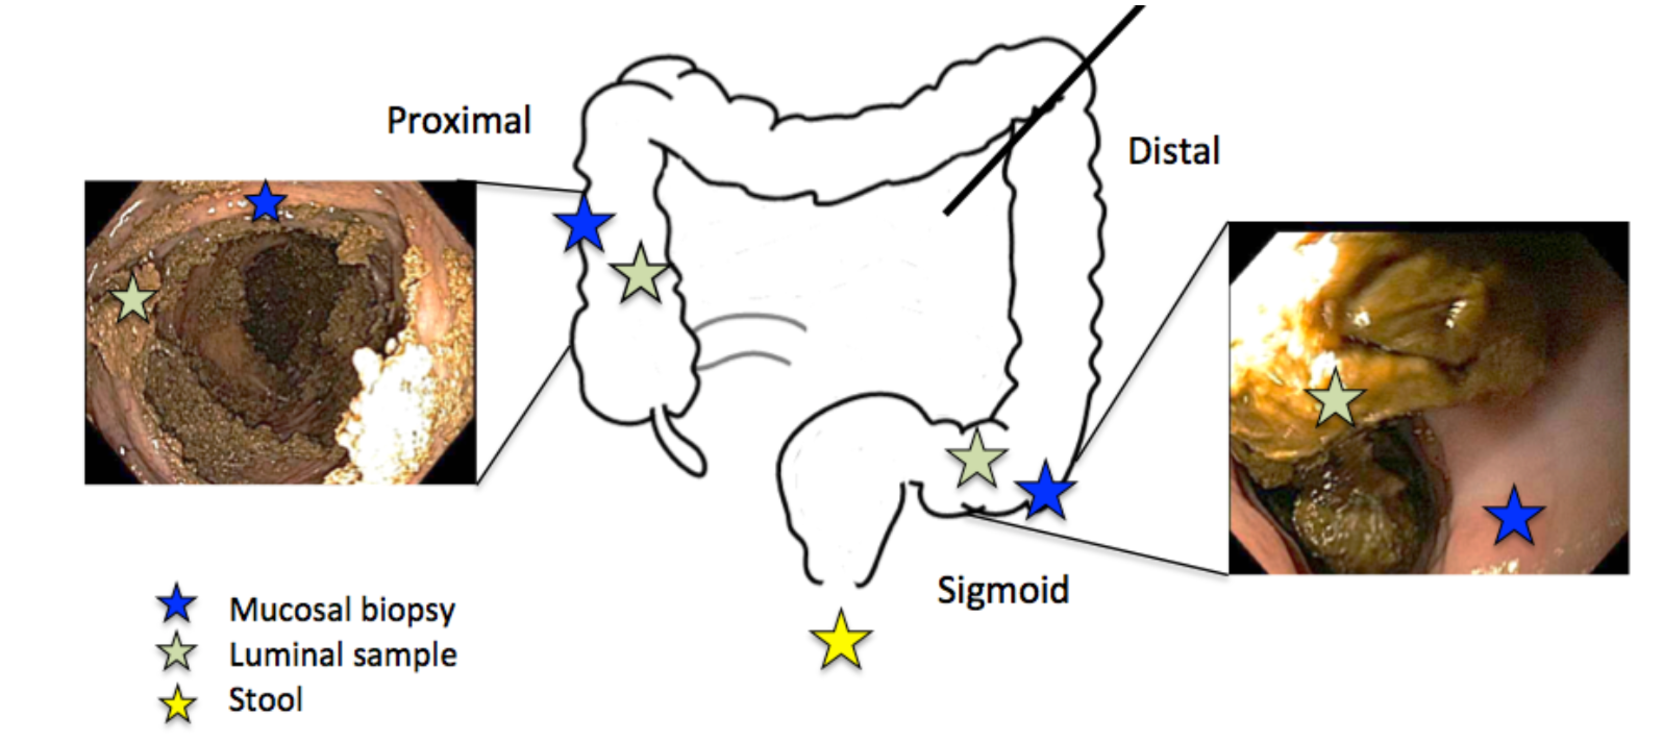
\includegraphics{submission/figure_1.pdf}

\paragraph{Figure 1}\label{figure-1}

Sampling strategy. A flexible sigmoidoscope was used to sample the
distal colonic luminal contents and mucosa. The scope was inserted
\textasciitilde{} 25cm into the subject and endoscopy brushes were used
to sample the luminal contents (green star). A separate set of biopsy
forceps was used to sample the distal mucosa (blue star). The
sigmoidoscope was removed. A pediatric colonoscope was inserted and used
to access the proximal colon. Biopsies were taken of the proximal
luminal contents and mucosa as described. One week prior to the
procedure stool was collected at home and sent into the laboratory.
Representative images from one individual are shown.

\newpage

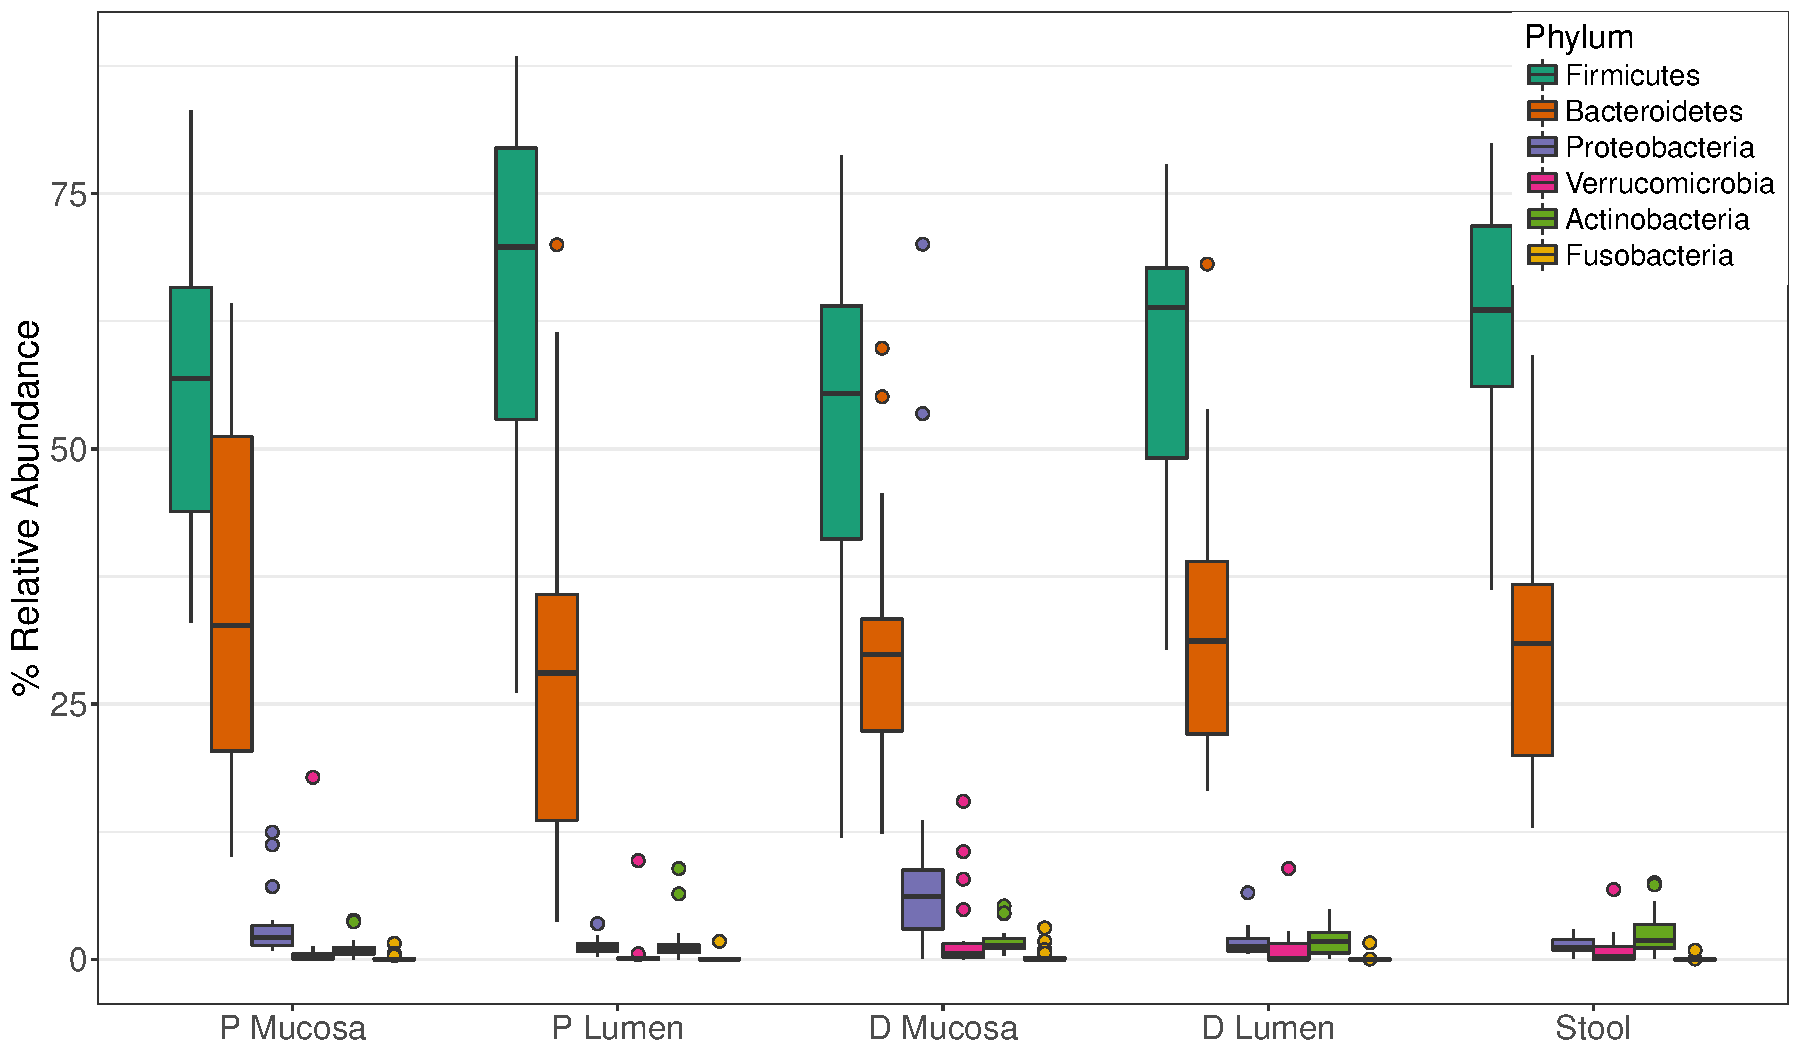
\includegraphics{submission/figure_2.pdf}

\paragraph{Figure 2}\label{figure-2}

Microbial membership and diversity of the proximal and distal human
colon. A) Relative abundance of the top five bacterial phyla in each
sampling site. Each box represents the median and confidence intervals.
B) Simpson diversity of the microbial communities at each location. The
lines represent the median values.

\newpage

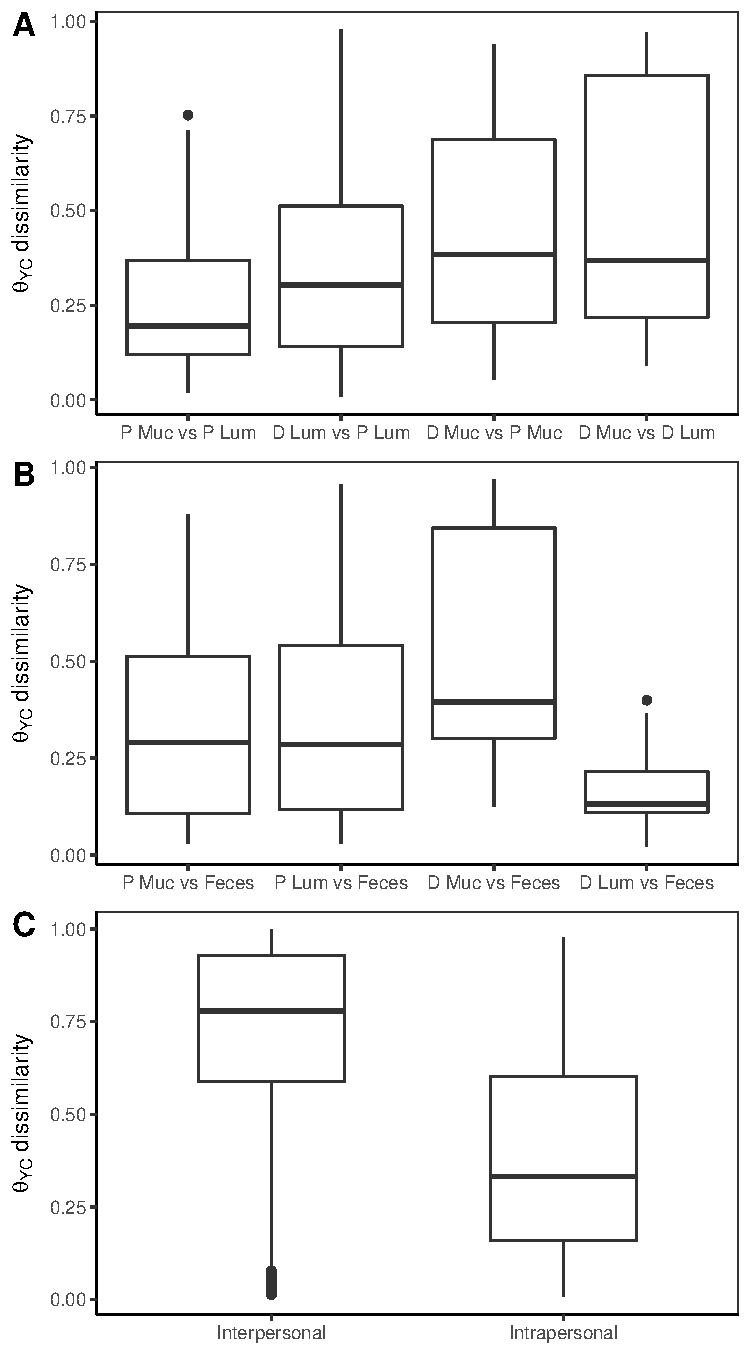
\includegraphics{submission/figure_3.pdf}

\paragraph{Figure 3}\label{figure-3}

Similarity of microbial community structure between sites of the gut.
ThetaYC distances are shown for interpersonal similarities between two
sites -- each point represents one individual. In (A), comparisons of
the right and left mucosal and lumen are shown. In (B), comparisons of
each site to the exit stool are shown.

\newpage

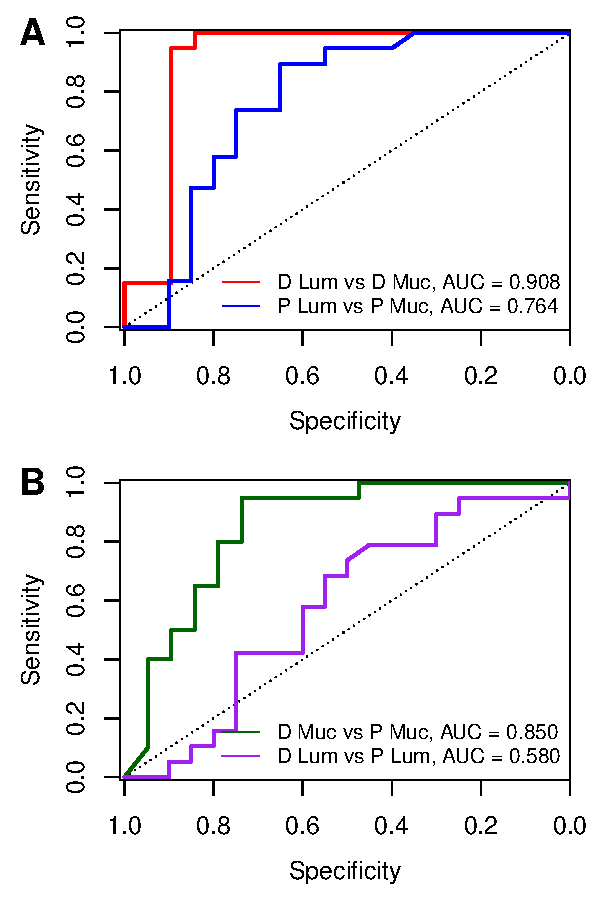
\includegraphics{submission/figure_4.pdf}

\paragraph{Figure 4}\label{figure-4}

Random Forest classifies the mucosa and lumen of each side of the colon.
A) Receiver Operator Characteristic curves are shown for the 10-fold
cross validation of the Random Forest model classifying lumen and
mucosal samples for the left and right sides of the colon. (B) Top five
OTUs that are most important for the classification model for the left
mucosa and lumen (B) and the right mucosa and lumen (C).

\newpage

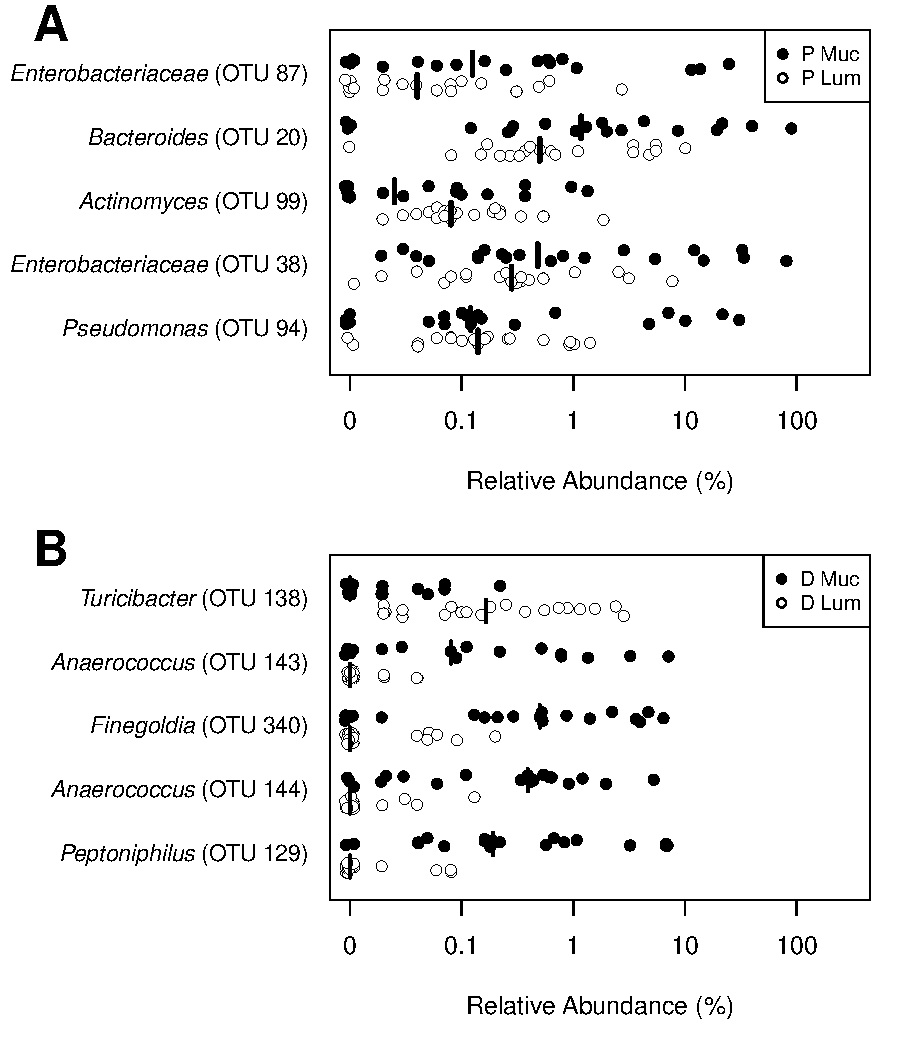
\includegraphics{submission/figure_5.pdf}

\paragraph{Figure 5}\label{figure-5}

Random Forest classifies the left and right sides of the colon. A)
Receiver Operator Characteristic curves are shown for the 10-fold cross
validation of the Random Forest model classifying left lumen versus
right lumen (orange) and left mucosa vs right mucosa (green). (B) Top
five OTUs that are most important for the classification model for the
left and right mucosa (B) and the left and right lumen (C).

\newpage

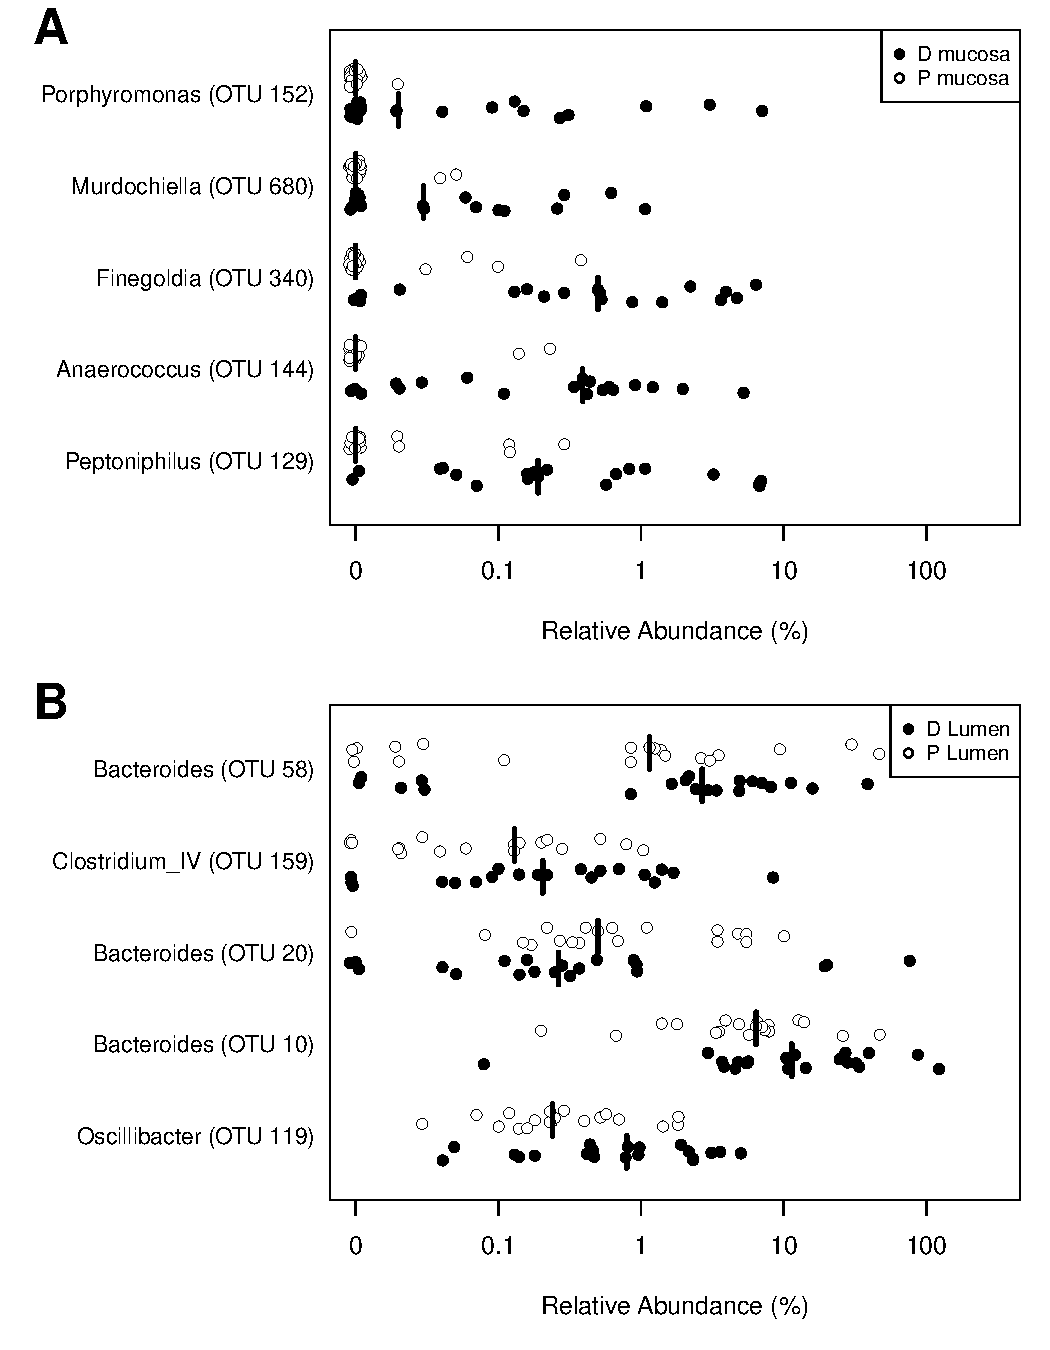
\includegraphics{submission/figure_6.pdf}

\paragraph{Figure 6}\label{figure-6}

Location and abundance of cancer-associated OTUs. Relative abundance was
calculated and plotted by sample site for each OTU of interest: (A)
\emph{Fusobacterium nucleatum} and (B) \emph{Porphyromonas
asacharolytica}

\subsubsection*{References}\label{references}
\addcontentsline{toc}{subsubsection}{References}

\hypertarget{refs}{}
\hypertarget{ref-Guinney2015}{}
1. \textbf{Guinney J}, \textbf{Dienstmann R}, \textbf{Wang X},
\textbf{Reyniès A de}, \textbf{Schlicker A}, \textbf{Soneson C},
\textbf{Marisa L}, \textbf{Roepman P}, \textbf{Nyamundanda G},
\textbf{Angelino P}, \textbf{Bot BM}, \textbf{Morris JS}, \textbf{Simon
IM}, \textbf{Gerster S}, \textbf{Fessler E}, \textbf{Melo FDSE},
\textbf{Missiaglia E}, \textbf{Ramay H}, \textbf{Barras D},
\textbf{Homicsko K}, \textbf{Maru D}, \textbf{Manyam GC}, \textbf{Broom
B}, \textbf{Boige V}, \textbf{Perez-Villamil B}, \textbf{Laderas T},
\textbf{Salazar R}, \textbf{Gray JW}, \textbf{Hanahan D},
\textbf{Tabernero J}, \textbf{Bernards R}, \textbf{Friend SH},
\textbf{Laurent-Puig P}, \textbf{Medema JP}, \textbf{Sadanandam A},
\textbf{Wessels L}, \textbf{Delorenzi M}, \textbf{Kopetz S},
\textbf{Vermeulen L}, \textbf{Tejpar S}. 2015. The consensus molecular
subtypes of colorectal cancer. Nature Medicine \textbf{21}:1350--1356.
doi:\href{https://doi.org/10.1038/nm.3967}{10.1038/nm.3967}.

\hypertarget{ref-Benedix2010}{}
2. \textbf{Benedix F}, \textbf{Kube R}, \textbf{Meyer F},
\textbf{Schmidt U}, \textbf{Gastinger I}, \textbf{Lippert H}. 2010.
Comparison of 17, 641 patients with right- and left-sided colon cancer:
Differences in epidemiology, perioperative course, histology, and
survival. Diseases of the Colon \& Rectum \textbf{53}:57--64.
doi:\href{https://doi.org/10.1007/dcr.0b013e3181c703a4}{10.1007/dcr.0b013e3181c703a4}.

\hypertarget{ref-Yamauchi2012}{}
3. \textbf{Yamauchi M}, \textbf{Lochhead P}, \textbf{Morikawa T},
\textbf{Huttenhower C}, \textbf{Chan AT}, \textbf{Giovannucci E},
\textbf{Fuchs C}, \textbf{Ogino S}. 2012. Colorectal cancer: A tale of
two sides or a continuum?: Figure 1. Gut \textbf{61}:794--797.
doi:\href{https://doi.org/10.1136/gutjnl-2012-302014}{10.1136/gutjnl-2012-302014}.

\hypertarget{ref-Albenberg2014}{}
4. \textbf{Albenberg L}, \textbf{Esipova TV}, \textbf{Judge CP},
\textbf{Bittinger K}, \textbf{Chen J}, \textbf{Laughlin A},
\textbf{Grunberg S}, \textbf{Baldassano RN}, \textbf{Lewis JD},
\textbf{Li H}, \textbf{Thom SR}, \textbf{Bushman FD}, \textbf{Vinogradov
SA}, \textbf{Wu GD}. 2014. Correlation between intraluminal oxygen
gradient and radial partitioning of intestinal microbiota.
Gastroenterology \textbf{147}:1055--1063.e8.
doi:\href{https://doi.org/10.1053/j.gastro.2014.07.020}{10.1053/j.gastro.2014.07.020}.

\hypertarget{ref-Donaldson2015}{}
5. \textbf{Donaldson GP}, \textbf{Lee SM}, \textbf{Mazmanian SK}. 2015.
Gut biogeography of the bacterial microbiota. Nature Reviews
Microbiology \textbf{14}:20--32.
doi:\href{https://doi.org/10.1038/nrmicro3552}{10.1038/nrmicro3552}.

\hypertarget{ref-Zackular2014}{}
6. \textbf{Zackular JP}, \textbf{Rogers MAM}, \textbf{Ruffin MT},
\textbf{Schloss PD}. 2014. The human gut microbiome as a screening tool
for colorectal cancer. Cancer Prevention Research \textbf{7}:1112--1121.
doi:\href{https://doi.org/10.1158/1940-6207.capr-14-0129}{10.1158/1940-6207.capr-14-0129}.

\hypertarget{ref-Zackular2013}{}
7. \textbf{Zackular JP}, \textbf{Baxter NT}, \textbf{Iverson KD},
\textbf{Sadler WD}, \textbf{Petrosino JF}, \textbf{Chen GY},
\textbf{Schloss PD}. 2013. The gut microbiome modulates colon
tumorigenesis. mBio \textbf{4}:e00692--13--e00692--13.
doi:\href{https://doi.org/10.1128/mbio.00692-13}{10.1128/mbio.00692-13}.

\hypertarget{ref-Dejea2014}{}
8. \textbf{Dejea CM}, \textbf{Wick EC}, \textbf{Hechenbleikner EM},
\textbf{White JR}, \textbf{Welch JLM}, \textbf{Rossetti BJ},
\textbf{Peterson SN}, \textbf{Snesrud EC}, \textbf{Borisy GG},
\textbf{Lazarev M}, \textbf{Stein E}, \textbf{Vadivelu J},
\textbf{Roslani AC}, \textbf{Malik AA}, \textbf{Wanyiri JW}, \textbf{Goh
KL}, \textbf{Thevambiga I}, \textbf{Fu K}, \textbf{Wan F}, \textbf{Llosa
N}, \textbf{Housseau F}, \textbf{Romans K}, \textbf{Wu X},
\textbf{McAllister FM}, \textbf{Wu S}, \textbf{Vogelstein B},
\textbf{Kinzler KW}, \textbf{Pardoll DM}, \textbf{Sears CL}. 2014.
Microbiota organization is a distinct feature of proximal colorectal
cancers. Proceedings of the National Academy of Sciences
\textbf{111}:18321--18326.
doi:\href{https://doi.org/10.1073/pnas.1406199111}{10.1073/pnas.1406199111}.

\hypertarget{ref-Baxter2016}{}
9. \textbf{Baxter NT}, \textbf{Ruffin MT}, \textbf{Rogers MAM},
\textbf{Schloss PD}. 2016. Microbiota-based model improves the
sensitivity of fecal immunochemical test for detecting colonic lesions.
Genome Medicine \textbf{8}.
doi:\href{https://doi.org/10.1186/s13073-016-0290-3}{10.1186/s13073-016-0290-3}.

\hypertarget{ref-Jalanka2014}{}
10. \textbf{Jalanka J}, \textbf{Salonen A}, \textbf{Salojärvi J},
\textbf{Ritari J}, \textbf{Immonen O}, \textbf{Marciani L},
\textbf{Gowland P}, \textbf{Hoad C}, \textbf{Garsed K}, \textbf{Lam C},
\textbf{Palva A}, \textbf{Spiller RC}, \textbf{Vos WM de}. 2014. Effects
of bowel cleansing on the intestinal microbiota. Gut
\textbf{64}:1562--1568.
doi:\href{https://doi.org/10.1136/gutjnl-2014-307240}{10.1136/gutjnl-2014-307240}.

\hypertarget{ref-Harrell2012}{}
11. \textbf{Harrell L}, \textbf{Wang Y}, \textbf{Antonopoulos D},
\textbf{Young V}, \textbf{Lichtenstein L}, \textbf{Huang Y},
\textbf{Hanauer S}, \textbf{Chang E}. 2012. Standard colonic lavage
alters the natural state of mucosal-associated microbiota in the human
colon. PLoS ONE \textbf{7}:e32545.
doi:\href{https://doi.org/10.1371/journal.pone.0032545}{10.1371/journal.pone.0032545}.

\hypertarget{ref-deCarcer2010}{}
12. \textbf{Cárcer DA de}, \textbf{Cuív PÓ}, \textbf{Wang T},
\textbf{Kang S}, \textbf{Worthley D}, \textbf{Whitehall V},
\textbf{Gordon I}, \textbf{McSweeney C}, \textbf{Leggett B},
\textbf{Morrison M}. 2010. Numerical ecology validates a biogeographical
distribution and gender-based effect on mucosa-associated bacteria along
the human colon. The ISME Journal \textbf{5}:801--809.
doi:\href{https://doi.org/10.1038/ismej.2010.177}{10.1038/ismej.2010.177}.

\hypertarget{ref-Zhang2013}{}
13. \textbf{Zhang Z}, \textbf{Geng J}, \textbf{Tang X}, \textbf{Fan H},
\textbf{Xu J}, \textbf{Wen X}, \textbf{Ma Z (Sam)}, \textbf{Shi P}.
2013. Spatial heterogeneity and co-occurrence patterns of human
mucosal-associated intestinal microbiota. The ISME Journal
\textbf{8}:881--893.
doi:\href{https://doi.org/10.1038/ismej.2013.185}{10.1038/ismej.2013.185}.

\hypertarget{ref-Castellarin2011}{}
14. \textbf{Castellarin M}, \textbf{Warren RL}, \textbf{Freeman JD},
\textbf{Dreolini L}, \textbf{Krzywinski M}, \textbf{Strauss J},
\textbf{Barnes R}, \textbf{Watson P}, \textbf{Allen-Vercoe E},
\textbf{Moore RA}, \textbf{Holt RA}. 2011. Fusobacterium nucleatum
infection is prevalent in human colorectal carcinoma. Genome Research
\textbf{22}:299--306.
doi:\href{https://doi.org/10.1101/gr.126516.111}{10.1101/gr.126516.111}.

\hypertarget{ref-Hong2011}{}
15. \textbf{Hong P-Y}, \textbf{Croix JA}, \textbf{Greenberg E},
\textbf{Gaskins HR}, \textbf{Mackie RI}. 2011. Pyrosequencing-based
analysis of the mucosal microbiota in healthy individuals reveals
ubiquitous bacterial groups and micro-heterogeneity. PLoS ONE
\textbf{6}:e25042.
doi:\href{https://doi.org/10.1371/journal.pone.0025042}{10.1371/journal.pone.0025042}.

\hypertarget{ref-Stearns2011}{}
16. \textbf{Stearns JC}, \textbf{Lynch MDJ}, \textbf{Senadheera DB},
\textbf{Tenenbaum HC}, \textbf{Goldberg MB}, \textbf{Cvitkovitch DG},
\textbf{Croitoru K}, \textbf{Moreno-Hagelsieb G}, \textbf{Neufeld JD}.
2011. Bacterial biogeography of the human digestive tract. Scientific
Reports \textbf{1}.
doi:\href{https://doi.org/10.1038/srep00170}{10.1038/srep00170}.

\hypertarget{ref-Sears2014}{}
17. \textbf{Sears CL}, \textbf{Garrett WS}. 2014. Microbes, microbiota,
and colon cancer. Cell Host \& Microbe \textbf{15}:317--328.
doi:\href{https://doi.org/10.1016/j.chom.2014.02.007}{10.1016/j.chom.2014.02.007}.

\hypertarget{ref-Mima2016}{}
18. \textbf{Mima K}, \textbf{Cao Y}, \textbf{Chan AT}, \textbf{Qian ZR},
\textbf{Nowak JA}, \textbf{Masugi Y}, \textbf{Shi Y}, \textbf{Song M},
\textbf{Silva A da}, \textbf{Gu M}, \textbf{Li W}, \textbf{Hamada T},
\textbf{Kosumi K}, \textbf{Hanyuda A}, \textbf{Liu L}, \textbf{Kostic
AD}, \textbf{Giannakis M}, \textbf{Bullman S}, \textbf{Brennan CA},
\textbf{Milner DA}, \textbf{Baba H}, \textbf{Garraway LA},
\textbf{Meyerhardt JA}, \textbf{Garrett WS}, \textbf{Huttenhower C},
\textbf{Meyerson M}, \textbf{Giovannucci EL}, \textbf{Fuchs CS},
\textbf{Nishihara R}, \textbf{Ogino S}. 2016. Fusobacterium nucleatum in
colorectal carcinoma tissue according to tumor location. Clinical and
Translational Gastroenterology \textbf{7}:e200.
doi:\href{https://doi.org/10.1038/ctg.2016.53}{10.1038/ctg.2016.53}.

\hypertarget{ref-Whitmore2014}{}
19. \textbf{Whitmore SE}, \textbf{Lamont RJ}. 2014. Oral bacteria and
cancer. PLoS Pathogens \textbf{10}:e1003933.
doi:\href{https://doi.org/10.1371/journal.ppat.1003933}{10.1371/journal.ppat.1003933}.

\hypertarget{ref-Flynn2016}{}
20. \textbf{Flynn KJ}, \textbf{Baxter NT}, \textbf{Schloss PD}. 2016.
Metabolic and community synergy of oral bacteria in colorectal cancer.
mSphere \textbf{1}:e00102--16.
doi:\href{https://doi.org/10.1128/msphere.00102-16}{10.1128/msphere.00102-16}.

\hypertarget{ref-Shobar2016}{}
21. \textbf{Shobar RM}, \textbf{Velineni S}, \textbf{Keshavarzian A},
\textbf{Swanson G}, \textbf{DeMeo MT}, \textbf{Melson JE},
\textbf{Losurdo J}, \textbf{Engen PA}, \textbf{Sun Y}, \textbf{Koenig
L}, \textbf{Mutlu EA}. 2016. The effects of bowel preparation on
microbiota-related metrics differ in health and in inflammatory bowel
disease and for the mucosal and luminal microbiota compartments.
Clinical and Translational Gastroenterology \textbf{7}:e143.
doi:\href{https://doi.org/10.1038/ctg.2015.54}{10.1038/ctg.2015.54}.

\hypertarget{ref-Kozich2013}{}
22. \textbf{Kozich JJ}, \textbf{Westcott SL}, \textbf{Baxter NT},
\textbf{Highlander SK}, \textbf{Schloss PD}. 2013. Development of a
dual-index sequencing strategy and curation pipeline for analyzing
amplicon sequence data on the MiSeq illumina sequencing platform.
Applied and Environmental Microbiology \textbf{79}:5112--5120.
doi:\href{https://doi.org/10.1128/aem.01043-13}{10.1128/aem.01043-13}.

\hypertarget{ref-Schloss2009}{}
23. \textbf{Schloss PD}, \textbf{Westcott SL}, \textbf{Ryabin T},
\textbf{Hall JR}, \textbf{Hartmann M}, \textbf{Hollister EB},
\textbf{Lesniewski RA}, \textbf{Oakley BB}, \textbf{Parks DH},
\textbf{Robinson CJ}, \textbf{Sahl JW}, \textbf{Stres B},
\textbf{Thallinger GG}, \textbf{Horn DJV}, \textbf{Weber CF}. 2009.
Introducing mothur: Open-source, platform-independent,
community-supported software for describing and comparing microbial
communities. Applied and Environmental Microbiology
\textbf{75}:7537--7541.
doi:\href{https://doi.org/10.1128/aem.01541-09}{10.1128/aem.01541-09}.

\hypertarget{ref-Wang2007}{}
24. \textbf{Wang Q}, \textbf{Garrity GM}, \textbf{Tiedje JM},
\textbf{Cole JR}. 2007. Naive bayesian classifier for rapid assignment
of rRNA sequences into the new bacterial taxonomy. Applied and
Environmental Microbiology \textbf{73}:5261--5267.
doi:\href{https://doi.org/10.1128/aem.00062-07}{10.1128/aem.00062-07}.

\hypertarget{ref-Liaw2002}{}
25. \textbf{Liaw A}, \textbf{Wiener M}. 2002. Classification and
regression by randomForest. R News: The Newsletter of the R Project
\textbf{2}:18--22.


\end{document}
